\documentclass{article}
\usepackage[12pt]{extsizes}
\usepackage[T2A]{fontenc}
\usepackage[utf8]{inputenc}
\usepackage[english, russian]{babel}

\usepackage{amssymb}
\usepackage{amsfonts}
\usepackage{amsmath}
\usepackage{enumitem}
\usepackage{graphics}
\usepackage{graphicx}

\usepackage{lipsum}

\newcommand{\definebox}[3]{%
	\newcounter{#1}
	\newenvironment{#1}[1][]{%
		\stepcounter{#1}%
		\mdfsetup{%
			frametitle={%
				\tikz[baseline=(current bounding box.east),outer sep=0pt]
				\node[anchor=east,rectangle,fill=white]
				{\strut #2~\csname the#1\endcsname\ifstrempty{##1}{}{##1}};}}%
		\mdfsetup{innertopmargin=1pt,linecolor=#3,%
			linewidth=3pt,topline=true,
			frametitleaboveskip=\dimexpr-\ht\strutbox\relax,}%
		\begin{mdframed}[]\relax%
		}{\end{mdframed}}%
}

\definebox{definition}{Определение}{blue!24}
\definebox{task}{Задача}{orange!24}

\usepackage{geometry} % Меняем поля страницы
\geometry{left=1cm}% левое поле
\geometry{right=1cm}% правое поле
\geometry{top=1.5cm}% верхнее поле
\geometry{bottom=1cm}% нижнее поле


\usepackage{fancyhdr} % Headers and footers
\pagestyle{fancy} % All pages have headers and footers
\fancyhead{} % Blank out the default header
\fancyfoot{} % Blank out the default footer
\fancyhead[L]{ЦРОД $\bullet$ Математика}
\fancyhead[C]{\textit{Методы}}
\fancyhead[R]{ЛФМШ 2023}% Custom header text


%----------------------------------------------------------------------------------------

%\begin{document}\normalsize
\begin{document}\large


\begin{center}
\textbf{Индукция}
\end{center}

\begin{enumerate}[label*=\protect\fbox{\arabic{enumi}}]
	
	\setcounter{enumi}{-3}
\begin{minipage}{0.5\linewidth}
	\item В клетке $A$ фигуры на рисунке стоит шахматный конь. Он должен дойти до клетки $B$. Ему нельзя быть ни в какой клетке дважды, а серые клетки он должен пройти все и строго слева направо по порядку. Придумайте маршрут и посчитайте число ходов.
\end{minipage}
\begin{minipage}{0.5\linewidth}
	\center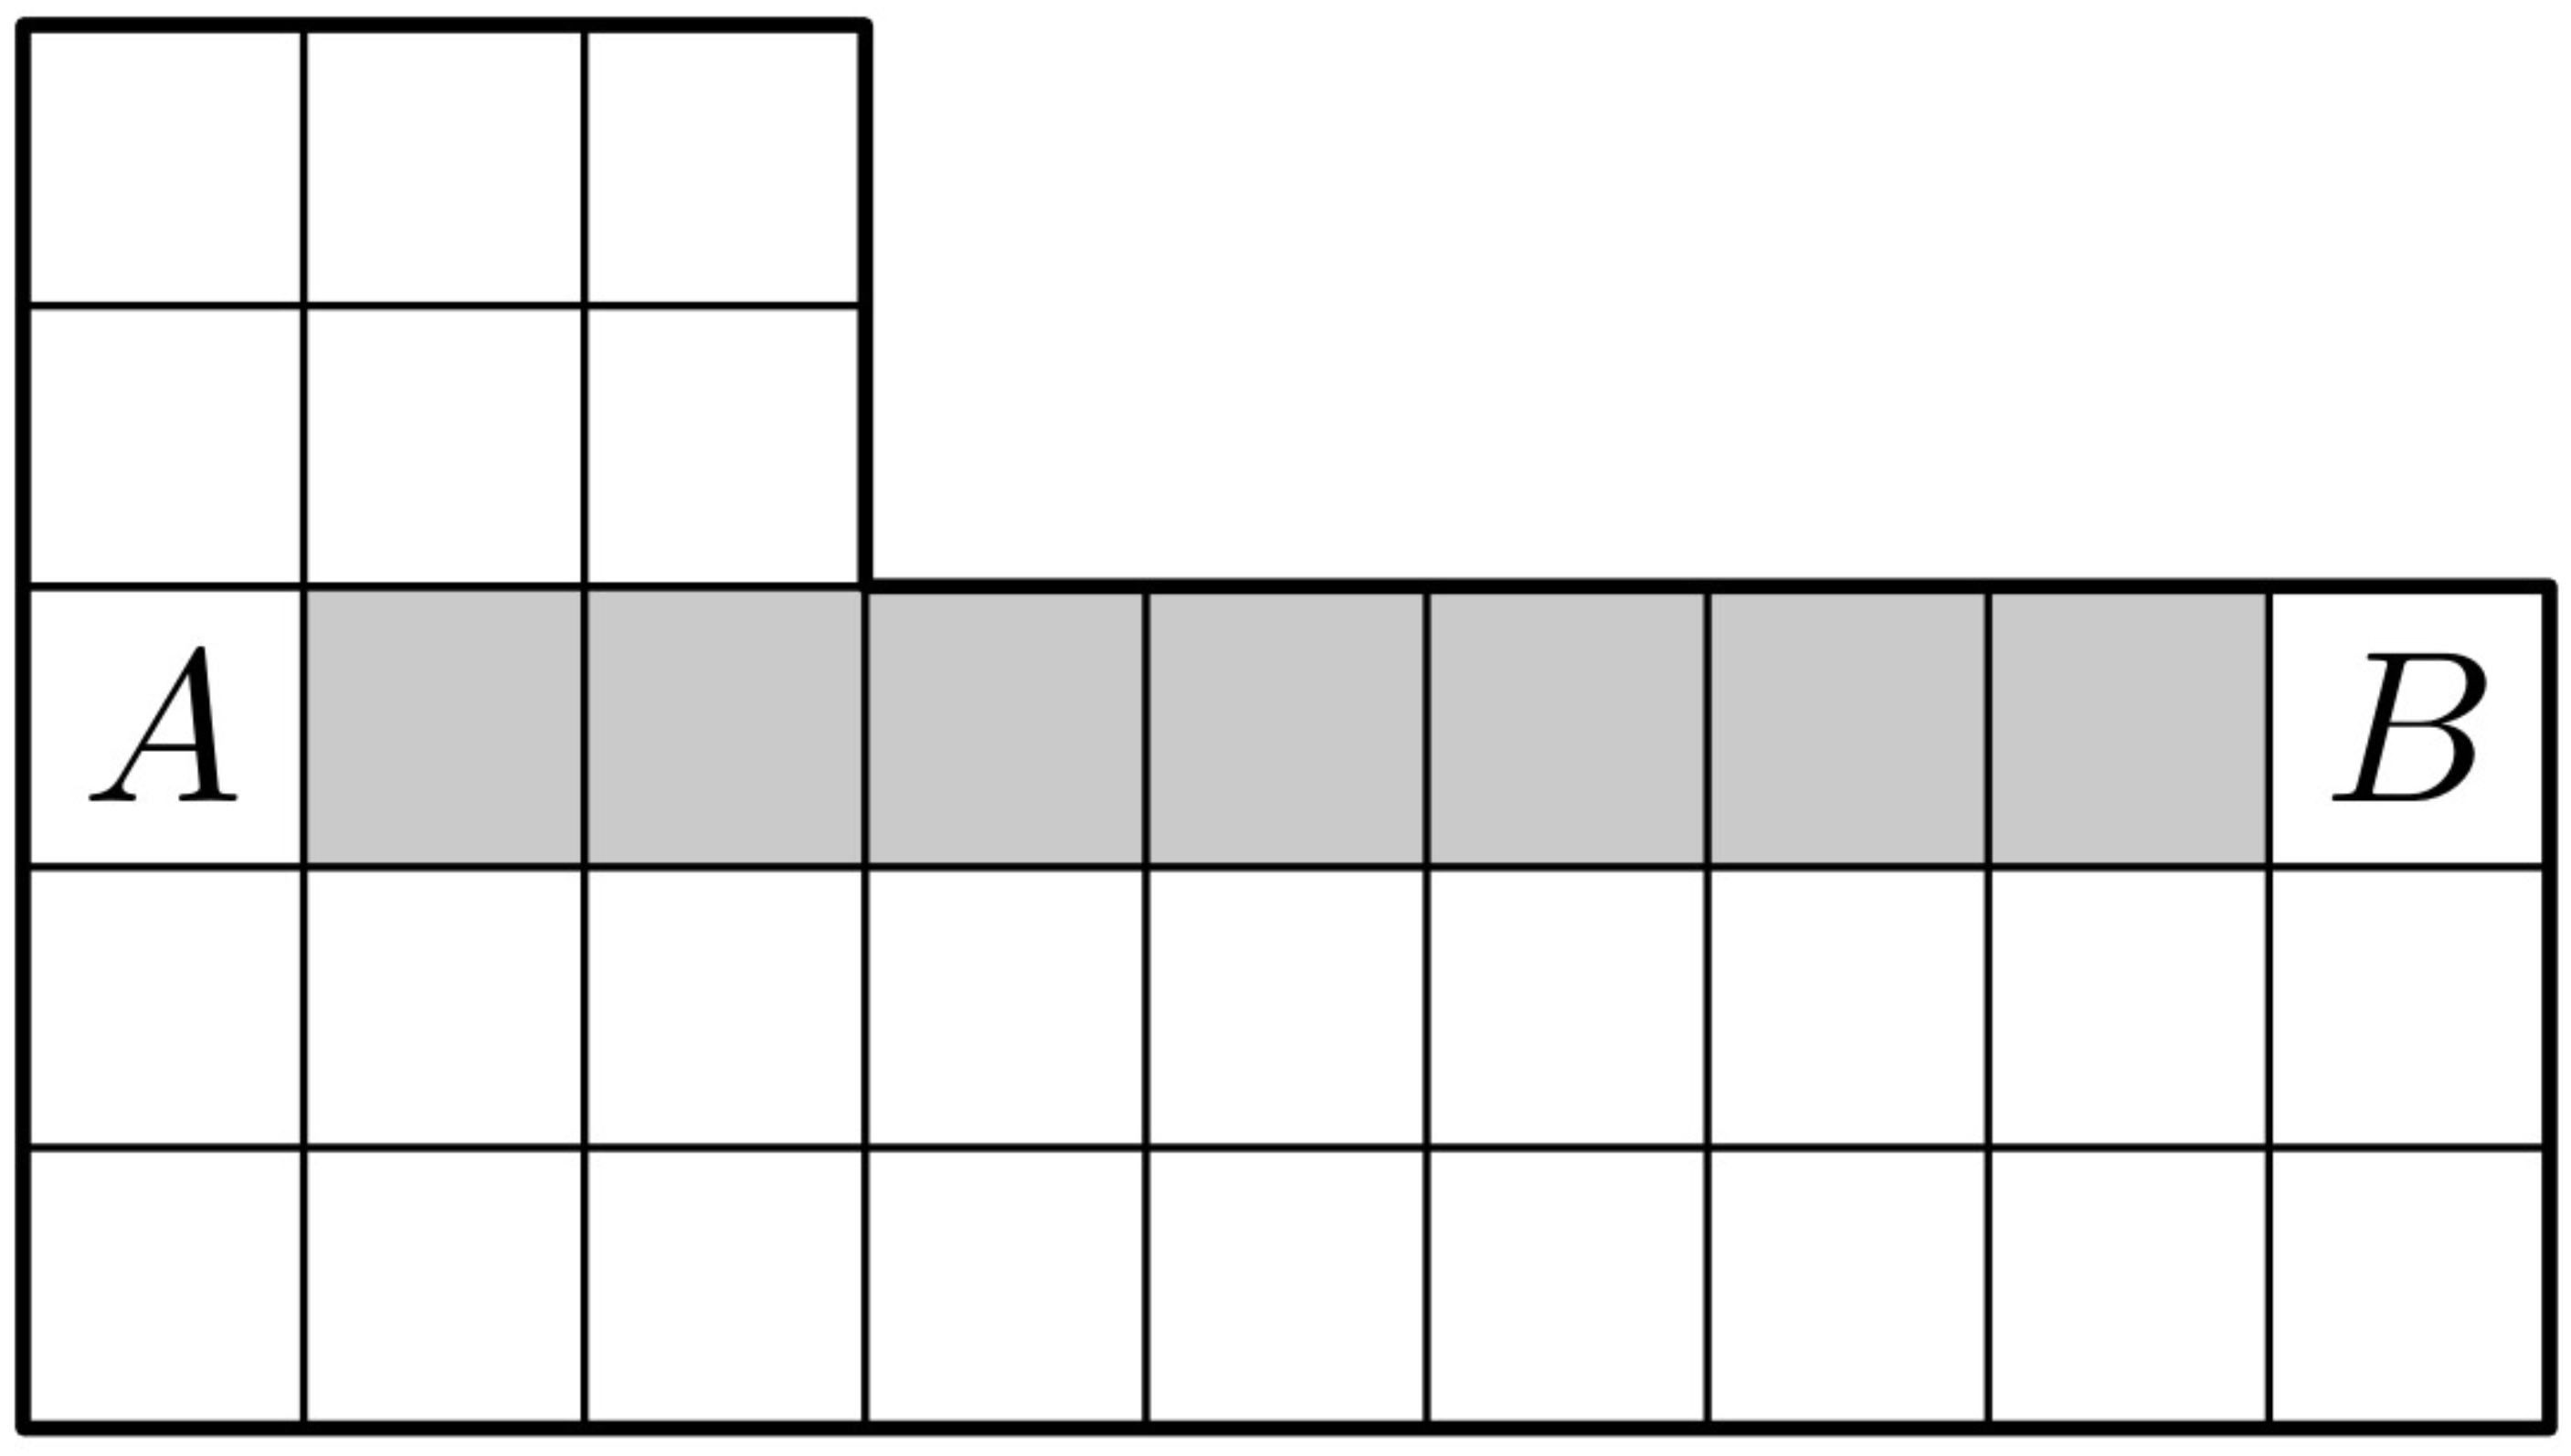
\includegraphics[width=0.7\textwidth]{img1.png}
\end{minipage}
\end{enumerate}


Часто требуется доказать утверждение типа:

\begin{center}
	\texttt{"Для каждого натурального $n$ докажите, что \dots"}.
\end{center}

Такое утверждение можно рассматривать, как цепочку утверждений 

\begin{center}
	\texttt{"Для $n = 1$ верно, что \dots"},
\end{center} 
\begin{center} 
	\texttt{"Для $n = 2$ верно, что \dots"} и т.д.
\end{center} 


Метод математической индукции состоит в том, чтобы доказать первое из этих утверждений (называемое \textbf{\textit{базой}} индукции), что обычно достаточно просто сделать, а затем доказать шаг (или \textbf{\textit{переход}}) индукции:
\begin{center} 
	\texttt{"Если верно утверждение с номером n, то и утверждение с номером (n + 1)"}.
\end{center} 

Если верна база индукции и верен шаг индукции, то все утверждения верны.

\begin{enumerate}[label*=\protect\fbox{\arabic{enumi}}]
	
\setcounter{enumi}{-2}
	
\item Докажите, что квадрат (a) $4 \times 4$; (b) $8 \times 8$; (c) $16 \times 16$; с вырезанной угловой клеткой можно разрезать на уголки из трех клеток.

\item Решите предыдущую задачу для квадрата $2^n \times 2^n$ для произвольного $n$.

\item Таня рисует на клетчатой бумаге пирамидку: в первом сверху ярусе одна клетка, во втором — три, в третьем — пять, в четвёртом — семь, и так далее. Сколько всего клеточек будет в первых 20 ярусах пирамидки? А в 1000 ярусах?

\item  (Треугольные числа) Напишите строку из 10 различных натуральных чисел таких, чтобы сумма любых двух соседних была точным квадратом. \textit{Путь к решению.} Для двух чисел самое простое $\{\textbf{1}, \textbf{3}\}$. Для трех чисел достаточно приписать в конце число, дополняющее тройку до точного квадрата. Подходит 6: $\{1, \textbf{3}, \textbf{6}\}$.
\item Плоскость разделена 100 прямыми на области. С одной стороны от каждой прямой растет борода. Докажите, что есть область, все границы которой бородаты наружу.

\item Плоскость поделена на области несколькими прямыми. Докажите, что области можно раскрасить в  два цвета в шахматном порядке (чтобы соседние области имели разный цвет).

\item Докажите, что любую сумму начиная с 19 копеек можно уплатить монетами 3 и 10 копеек

\item Докажите, что $\underbrace{111\dots111}_{3^n}\;\vdots\; 3^n$ для любого натурального $n$

\item Для натуральных $n$ докажите, что $2^n > n$

\item Для натуральных $n \geqslant 4$ докажите, что $n! > 2^n$

\item \textit{Неравенство Бернулли}: $(1+a)^n\ge 1+an$, $n \in \mathbb{N}$, $a > - 1$

\item Известно, что  $x + \dfrac{1}{x}$  – целое число. Докажите, что  $x^n + \dfrac{1}{x^n}$  – также целое при любом натуральном $n$.

\item Проведём в выпуклом многоугольнике некоторые диагонали так, что никакие две из них не пересекаются (из одной вершины могут выходить несколько диагоналей). Доказать, что найдутся по крайней мере две вершины многоугольника, из которых не проведено ни одной диагонали. 

\item Даны два выпуклых многоугольника $A_1A_2A_3\dots A_n$ и $B_1B_2B_3\dots B_n$. Известно, что $A_1A_2 = B_1B_2, A_2A_3 = B_2B_3,\dots, A_nA_1 = B_nB_1$ и $n - 3$ угла одного многоугольника равны соответственным углам другого. Будут ли многоугольники равны?

\item Докажите, что любой квадрат можно разрезать на любое число квадратиков (не обязательно одинаковых), начиная с 6.

%\item Докажите по индукции, что
%\begin{enumerate}
%	\item $1 + 2 + \dots + n =\dfrac{n (n+1)}{2}$
%	
%	\item $1 + 3 + 5 + \dots + (2n - 1) = n^2$
%	
%	\item $1^2 + 2^2 + \dots + n^2 =\dfrac{n (n+1)(2n + 1)}{6}$
%	
%	\item $1 \cdot 2 + 2 \cdot 3 + 3 \cdot 4 + \dots + n(n + 1) = \dfrac{n(n + 1)(n+2)}{3}$
%	
%	\item $1^3 + 2^3 + \dots + n^3 =(1 + 2 + \dots + n) ^ 2$
%\end{enumerate}

\item Докажите, что $n^n \ge (n + 1)^{n - 1}$, $n \in \mathbb{N}$
\end{enumerate}
\end{document}